\documentclass[../main.tex]{subfiles}
\begin{document}
\setchapterstyle{kao}
\setchapterpreamble[u]{\margintoc}
\chapter[Lie groups I - fundamentals]{Lie groups I - fundamentals\footnotemark[0]}
\labch{Lie-groups-I}
\section{Definitions}
In few words, a Lie group is a group which is also a manifold in such a way that the two structures, namely the algebraic structure of the group and the differential structure of the manifold, \textit{interact well} with each other. \textit{To interact well} means that both the operations, one is sending two elements to their product and the other is the inversion, are smooth maps.
\begin{definition}[Lie Group]
A Lie group is a group $(G,\cdot)$ such that $G$ equipped with an atlas $A$, i.e. $(G,A)$, is a manifold and the following hold true:\marginnote{\underline{Recall Exercise:} If $M$ and $N$ are manifold, then $M\times N$ is a manifold.}
\begin{enumerate}
    \item
    \[
    \begin{split}
        G\times G &\to G\\
        (g,k)&\mapsto g\cdot k
    \end{split} \quad \textrm{is $C^{\infty}$\textbf{-smooth}}
    \]
    \item 
    \[
    \begin{split}
        G &\to G\\
        g&\mapsto g^{-1}
    \end{split} \quad \textrm{is $C^{\infty}$\textbf{-smooth}}
    \]
\end{enumerate}
\end{definition}
The fact that there are this two structure that interact well between each other, have some important consequences.
\section{Main features of a Lie groups}
\subsection[Operations are continuous]{Operations are continuous}
Those more interested in abstract theory, could ask <<Continuous in which sense?>> If our group is embedded in $\mathbb{R}^n$, there is no question: basically we inherit a notion of continuity from the embedding (the larger linear space). But suppose it is not, if $(G,A)$ is \underline{not} embedded in $\mathbb{R}^N$, in which sense should we understand \textbf{\textit{continuity}}?? Many relevant notion of Analysis 1 (continuity, compactness, connectedness, ...) are defined only by specifying the \textbf{\textit{family of open subsets}}.
\begin{definition}[Topology - Topologia]\index{Topology}
A \textbf{topology} $\pazocal{T}$ is a collection of subsets of $S$, i.e. $\pazocal{T}\subseteq \pazocal{P}(S)$\marginnote{\begin{kaobox}[frametitle=Note]
$\pazocal{P}(S)$ is the set of all subsets of $S$.
\end{kaobox}}
such that: 
\begin{enumerate}\renewcommand{\labelenumi}{(O\arabic{enumi})}
    \item \textbf{Finite intersections}
    \[\Bqty{O_1,\dots,O_n} \ \textrm{ open sets, then } \ \bigcap_{i=1}^n O_i \ \textrm{ is an open set}\]
    \item \textbf{Arbitrary unions}
    \[\Bqty{O_\alpha}_{\alpha\in A} \ \textrm{ , with $A$ arbitrary, then } \ \bigcup_{\alpha\in A} O_\alpha \ \textrm{ \textbf{is an open set}}\]
    \item The empty/void set $\emptyset$ and the full set $S$ are \textbf{open sets}.
\end{enumerate}
\end{definition}
We can axiomatize this:
\begin{definition}[\href{https://it.wikipedia.org/wiki/Spazio\_topologico\#Definizione\_tramite\_\%22aperti\%22}{Topological space}]\index{Topological space (via open sets)}
A \textbf{topological space} is a pair $(S,\pazocal{T})$, with $\pazocal{T}\subseteq \pazocal{P}(S)$, such that $\pazocal{T}$ satisfies (O1), (O2), (O3).
\end{definition}
Now we use that to give a topology to a manifold $\mathbf{M}$.
\begin{definition}
$(\mathbf{M}, A)$ is equipped with a topology $\pazocal{T}$, by the following:
\[
A \subseteq \mathbf{M} \ \textrm{ is in $\pazocal{T}$}
\]
if $\forall \ (\pazocal{U}_\alpha, \varphi_\alpha)\in A$ it happens that
\[
\varphi_\alpha^{-1}(A\cap \pazocal{U}_\alpha) \ \textrm{ is open in } \ \mathbb{R}^n
\]
\end{definition}
\begin{figure}[H]
	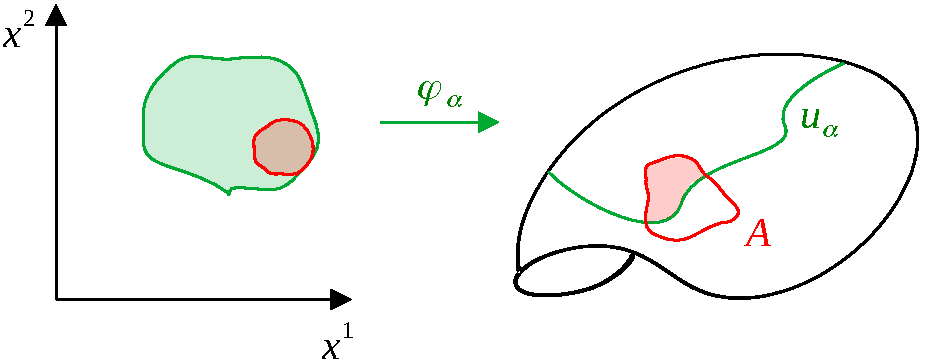
\includegraphics{images/top_space.pdf}
	\caption{Chart that maps from a subset of the local chart to our manifold.}
	\labfig{top-space}
\end{figure}
Looking at \reffig{top-space}, we declare that a set is open if for every chart, if we take the intersection of $A$ with the domain were the chart is defined and we pull it back via the chart, what we obtain is an open subset of $\mathbb{R}^n$.
\begin{kaobox}[frametitle=Remark]
If $(\mathbf{M}, A)$ is generic, the topology defined this way might be \textbf{\textit{pathological}} (Chapter 3 of \sidecite{doCarmo1994}). It will \underline{\underline{not}} happen in all the physically relevant examples (in this course, at least).
\end{kaobox}
\subsection{Infinitesimal structure of a Lie group}
This is more relevant for physics. Let us start with a picture that maybe is more important than the definition: \reffig{inf-struct-lie-group}.
\begin{figure}[h!]
	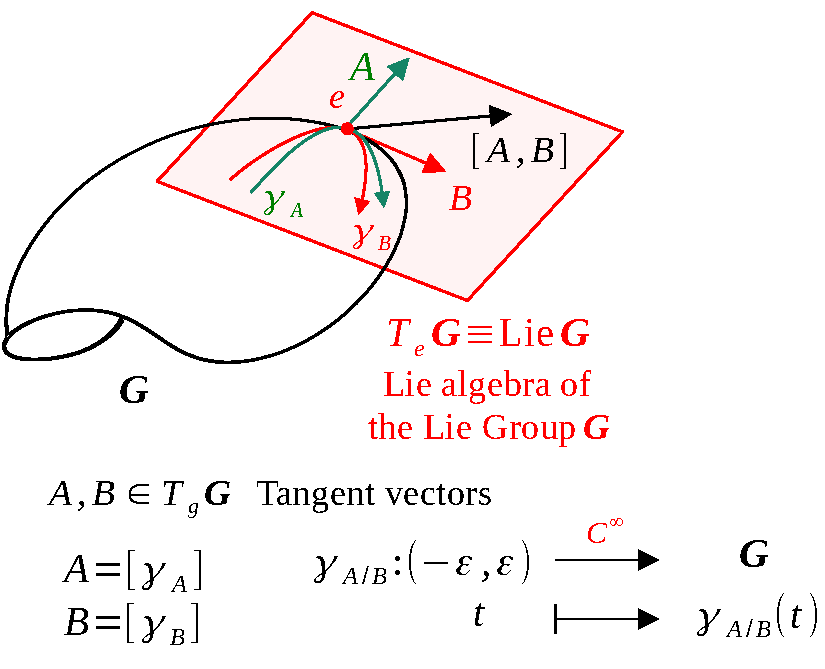
\includegraphics{images/inf-struct-lie-group.pdf}
	\caption{Lie algebra of the Lie group}
	\labfig{inf-struct-lie-group}
\end{figure}
This is the outline of the group $G$ (which is also a manifold) and it has a special point: the neutral element (or identity) $e$. All the tangent spaces are equal, but one is more equal than the others\marginnote{From George Orwell’s \href{https://en.wikipedia.org/wiki/Animal_Farm}{Animal Farm}: \textit{all
animals are equal but some animals are more
equal than others.}}: the tangent space at the identity, it is so important that is has its own name: the \textbf{\textit{Lie algebra of the Lie group}}\index{Lie algebra}. Why do we call it \textit{algebra} even if it is just a tangent space? Because it will become an algebra thanks to the fact that $G$ is a group.
\begin{itemize}
    \item If we take two tangents vector $A,B$ at the identity, of course if there is an embedding they will be like in the \reffig{inf-struct-lie-group}, but in general they will be equivalent classes of smooth maps $\gamma_A$ and $\gamma_B$.
    \item Now comes the magic: as $\gamma_A$ and $\gamma_B$ takes values in the group $G$, we can \underline{\textbf{multiply}} them and obtain a new path
    \[
    t \mapsto \gamma_A(t) {\color{red}\underset{\mathclap{\tikz \node {$\uparrow$} node [below=1ex] {\footnotesize in $G$ };}}{\cdot}}\gamma_B(t)
    \]
    which is still $C^\infty$\textbf{-smooth}\sidenote{since each one of the two is $C^\infty$-smooth and the composition, i.e. the operation in the group, is smooth itself by definition} and it is at $e\in G$ when $t=0$.
    \item We can also \textbf{invert}, and obtain a new path
    \[
    t \mapsto \gamma_A(t)^{-1} \quad (\textrm{or }\ \gamma_B(t)^{-1})
    \]
    which is $C^\infty$\textbf{-smooth} and  at $e\in G$ when $t=0$.
\end{itemize} 
To obtain the Lie algebra structure we have to combine the paths $\gamma_A, \gamma_B$ and their \textbf{inverses}. A rescaling of time is also needed. Now let us give a formal definition.\marginnote[30mm]{
\begin{kaobox}[frametitle=Remark]
This definition will be reconsidered later in the course.
\end{kaobox}}
\begin{definition}[Lie algebra structure on $T_eG$]\index{Lie algebra structure on $T_eG$}
Let $A,B\in T_eG$ such that $A=\bqty{a}$ and $B=\bqty{b}$\marginnote{$a,b$ were $\gamma_A,\gamma_B$ in the \reffig{inf-struct-lie-group}}. Consider the curve $c:(-\varepsilon,\varepsilon)\to G$ defined by:\marginnote{You can still check that $c(t)$ is smooth}
\[
c(t)=a(\sqrt{t})b(\sqrt{t})a(\sqrt{t})^{-1}b(\sqrt{t})^{-1}
\]
Then the Lie product of $A$ and $B$ is defined by:
\begin{equation}\labeq{lie-product}
    \comm{A}{B}:=\underset{\mathclap{\tikz \node {$\uparrow$} node [below=1ex] {\footnotesize Equivalence class in $K_e(G)$ };}}{\bqty{c}}=\dv{t}c(t)\big|_{t=0} \qquad \Big|\Big| \quad \star 
\end{equation}
\end{definition}
\begin{kaobox}[frametitle=Remark]
The reason of definition in \refeq{lie-product} will become clear later, when dealing with \textbf{matrix} Lie group (it will be a commutator!). To understand its \textit{spirit}, just consider the case
\[
\begin{split}
    a(t)&=e^{tA}=\mathbb{1}+tA+\frac{1}{2}t^2A^2+\pazocal{O}(t^3)\\
    b(t)&=e^{tB}=\mathbb{1}+tB+\frac{1}{2}t^2B^2+\pazocal{O}(t^3)
\end{split}
\]
and compute $\dv{t}c(t)\big|_{t=0}$. Here $A,B\in\textrm{Mat}(n,\mathbb{K})$.
\end{kaobox}
\begin{definition}[Lie algebra]\index{Lie algebra}\labdef{Lie-algebra}
A \textbf{Lie algebra} is a vector space $V$ equipped with a binary operation
\[
\begin{split}
    V\times V &\to V\\
    (v,w) &\mapsto [v,w]
\end{split}
\]
with the following properties:
\begin{enumerate}\renewcommand{\labelenumi}{(L\arabic{enumi})}
    \item Bilinear: $\forall \; \lambda_1,\lambda_2 \in \mathbb{R}^n \quad \forall\; v_1,v_2,w \in V$
    \[
    \begin{split}
        \comm{\lambda_1v_1+\lambda_2v_2}{w}&=\lambda_1\comm{v_1}{w}+\lambda_2\comm{v_2}{w}\\
        \comm{w}{\lambda_1v_1+\lambda_2v_2}&=\lambda_1\comm{w}{v_1}+\lambda_2\comm{w}{v_2}
    \end{split}
    \]
    \item \textbf{Anti-symmetric}: $\forall \ v,w\in V$
    \[
    \comm{w}{v}=\underset{\mathclap{\tikz \node {$\uparrow$} node [below=1ex] {\footnotesize Minus!};}}{-}\comm{v}{w}
    \]
    \item \textbf{Jacobi}:\marginnote{$\circlearrowright$ Cyclate!}
    \[
    \comm{v}{\comm{w}{z}}+\comm{z}{\comm{v}{w}}+\comm{w}{\comm{z}{v}}=0
    \]
\end{enumerate}
\end{definition}
This is a general structure and there are many examples of this structure.
\begin{marginfigure}[-175mm]
	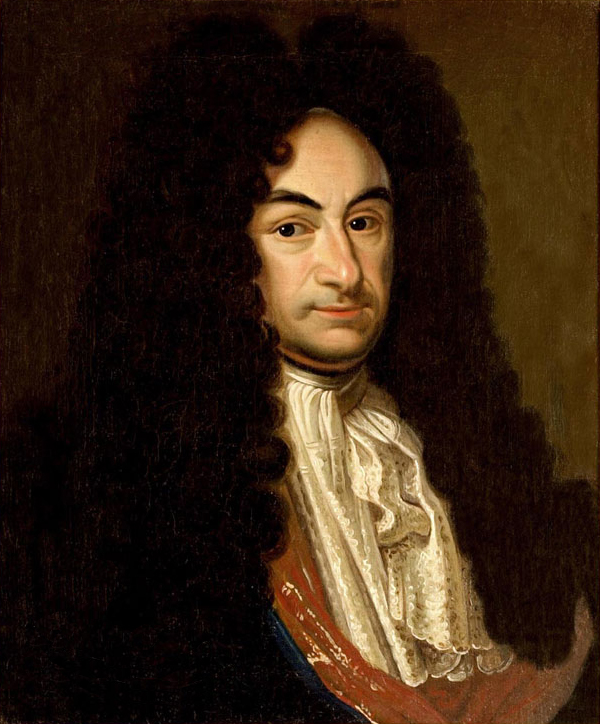
\includegraphics[width=1\linewidth]{images/Leibniz_Hannover.jpg}
	\caption[A portrait of Gottfried Wilhelm von Leibniz - Public Library of Hannover]{From \href{https://commons.wikimedia.org/wiki/File:Leibniz_Hannover.jpg}{Wikimedia}: A portrait of Gottfried Wilhelm von Leibniz - Public Library of Hannover (Lower Saxony). Gottfried Wilhelm (von) Leibniz (1 July 1646 [O.S. 21 June] – 14 November 1716) was a German polymath active as a mathematician, philosopher, scientist, and diplomat. He is a prominent figure in both the history of philosophy and the history of mathematics. Leibniz died in Hanover in 1716. At the time, he was so out of favor that neither George I (who happened to be near Hanover at that time) nor any fellow courtier other than his personal secretary attended the funeral. Even though Leibniz was a life member of the Royal Society and the Berlin Academy of Sciences, neither organization saw fit to honor his death. His grave went unmarked for more than 50 years. He was, however, eulogized by Fontenelle, before the French Academy of Sciences in Paris, which had admitted him as a foreign member in 1700. The eulogy was composed at the behest of the Duchess of Orleans, a niece of the Electress Sophia.}
	\labfig{Leibntiz}
\end{marginfigure}
\begin{example}
This should be already familiar. We take the endomorphism (or linear operator) of linear spaces as our vector space, namely $\textrm{End}(\mathbb{R})^n=:V$ and we define the product as the commutator
\[
\comm{A}{B}=AB-BA
\]
Moreover, it satisfies
\begin{enumerate}\renewcommand{\labelenumi}{(L4)}
    \item \underline{Leibniz:} $\comm{A}{BC}=\comm{A}{B}C+B\comm{A}{C}$
\end{enumerate}
We say that the operation is a derivation in the sense that satisfies the Leibniz property, if we define
\[
\delta_A(B)= \comm{A}{B} \ \Rightarrow \ \delta_A \textrm{ is a \textbf{derivation} on the algebra of $\textrm{End}(V)$}
\]
\end{example}
\begin{exercise}
Check that it is a Lie algebra.
\end{exercise}
Another example which is the same but extended to infinite dimension is the following.
\begin{marginfigure}
	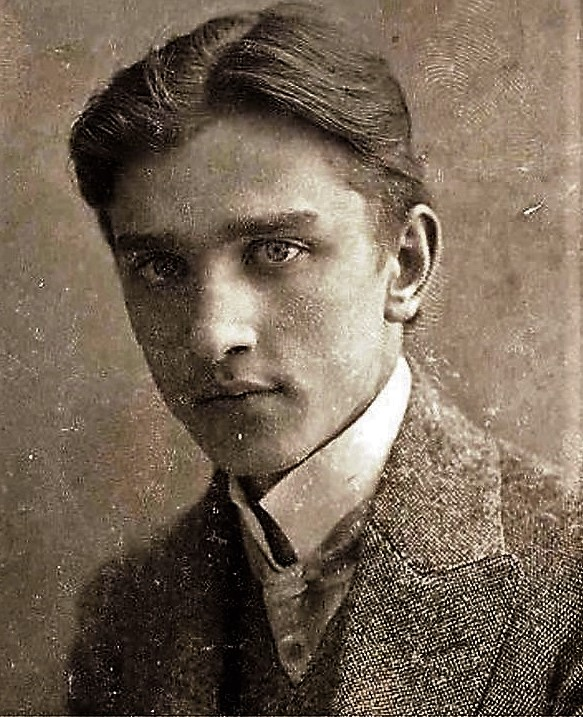
\includegraphics[width=1\linewidth]{images/Stefan_Banach.jpg}
	\caption[Photo of Stefan Banach in 1919]{From \href{https://commons.wikimedia.org/wiki/File:Stefan_Banach.jpg?uselang=it}{Wikimedia}: Stefan Banach in 1919. Stefan Banach (30 March 1892 – 31 August 1945) was a Polish mathematician who is generally considered one of the world's most important and influential 20th-century mathematicians. He was the founder of modern functional analysis, and an original member of the Lwów School of Mathematics. His major work was the 1932 book, \textit{Théorie des opérations linéaires} (Theory of Linear Operations), the first monograph on the general theory of functional analysis. After the Red Army recaptured Lviv in the Lvov–Sandomierz Offensive of 1944, Banach returned to the University and helped re-establish it after the war years. However, because the Soviets were removing Poles from annexed formerly Polish territories, Banach began preparing to leave the city and settle in Kraków, Poland, where he had been promised a chair at the Jagiellonian University. He was also considered a candidate for Minister of Education of Poland. In January 1945, he was diagnosed with lung cancer and was allowed to stay in Lwów. He died on 31 August 1945, aged 53. His funeral at the Lychakiv Cemetery was attended by hundreds of people.}
	\labfig{Banach}
\end{marginfigure}
\begin{example}
Take $E$ a Banach space / Hilbert space. Define out vector space to be the bounded operators on $E$, equipped with a product which is the same as before
\[
\begin{split}
    \pazocal{B}(E)&=:V\\
    \comm{A}{B}&=AB-BA
\end{split}
\]
\end{example}
\begin{exercise}
Check that is is a Lie algebra\footnote{Actually a infinite dimensional one, but actually we never asked to the vector space to be finite-dimensional.} with \textbf{Leibniz property} (L4).
\end{exercise}
\begin{starredExercise}
Check that, for any Lie group $G$, the \textbf{Lie algebra of the Lie group} is a Lie algebra, i.e. (L1), (L2) and (L3) are satisfied.
\end{starredExercise}
The previous exercise seems tautological because of the name, but actually when we define a Lie algebra of a Lie group we just define the product, we did not check it satisfies the properties. In this case we cannot even ask ourselves whether (L4) is satisfied or not, because we do not know in general what does it mean to take the product of two vector, unless we take the Lie product.
\begin{kaobox}[frametitle=Note]
The \textbf{\textit{concrete version}} of this exercise will appear when we will introduce the \textbf{matrix exponential}.
\end{kaobox}
\section{Examples of Lie groups}
Let us forget for a moment the algebra and go back to the groups.
\subsection{The king of all the examples}\labsubsec{king-of-exs}
This is the general linear group
\[
\textrm{GL}(\mathbb{R}^n)\equiv \textrm{GL}(n,\mathbb{R})= \Bqty{A\in \textrm{End}(\mathbb{R}^n): \ \exists \ A^{-1}\in\textrm{End}(\mathbb{R}^n)}
\]
It has a brother which is the complex case, but just to fix the idea we consider the real case.
\begin{proposition}
The general linear group equipped with the composition of endomorphisms (composition of linear operators) $(\textrm{GL}(\mathbb{R}^n), \circ )$ is a \textbf{Lie group}. Moreover, it admits a \textbf{global chart}.\marginnote{A single chart that will cover all the general linear group, which is syntomatic of the fact that, in a sense, is flat.}
\end{proposition}
\begin{figure}[h!]
	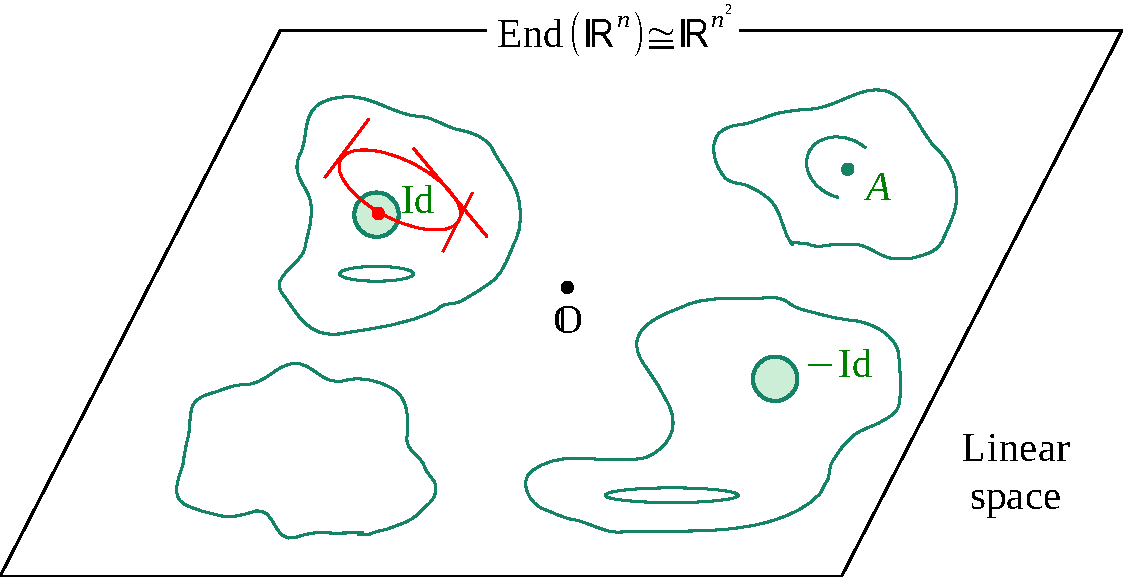
\includegraphics{images/Glob-chart-lie-group.pdf}
	\caption{Representation of the general linear group.}
	\labfig{king-of-ex}
\end{figure}
Why it happens like that? We have to pick that this group comes naturally inside a linear space (\reffig{king-of-ex}): the endomorphism of $\mathbb{R}^n$ is a linear space (which is flat by definition) which can be identified with $n\times n$ real matrices, so in the end it is isomorphic to $\mathbb{R}^{n^2}$. In this linear space of endomorphism there are some distinguish points: $\mathbb{0}$, which is definitely not invertible, and there is the trivial endomorphism: the identity $\mathbb{1}$ (or Id), which is invertible (there will be also $-\mathbb{1}$, which is also invertible). A general linear group is an open subset of linear space, that we do not know exactly how it is, (green lines in the picture). In particular it contains a neighbourhood of the identity and of minus the identity.
\begin{proof}
\begin{enumerate}
    \item $(\textrm{GL}(\mathbb{R}^n), \circ )$ is group (\vrefexample{general-linear-group} in \refch{groups-fund-conc})
    \item We need to check it is a manifold, actually we claim much more: $\textrm{GL}(\mathbb{R}^n)$ admits an atlas with only a chart. Reffering to \reffig{king-of-ex}, the global chart is:
    \[
    \begin{split}
        \varphi^{-1}: \textrm{GL}(\mathbb{R}^n)&\to \mathbb{R}^{n^2}\\
        A &\underset{\mathclap{\tikz \node {$\uparrow$} node [below=1ex] {\footnotesize choose a \textbf{linear bases $\Bqty{e_1,\dots,e_n}$} };}}{\mapsto} \pqty{A^i_{\;\;j}}=x^\mu(A)
    \end{split}
    \]
    where $\mu=(i,j)\in\Bqty{1,\dots,n}\times\Bqty{1,\dots,n}$.\sidenote{This is one of the few points were the Ricci's notation\index{Ricci's notation} does not work very well. In fact, if we look at $A$ as an endomorphism of $\mathbb{R}^n$, it makes sense to have the indices at different levels: because as an endomorphism is a tensor of type $\binom{1}{1}$. But if we look at $A$ as a point in the general linear group, since it is a point its coordinates have only the indices upstairs.}
    \sidenote{The chart is global by construction and is only one, so we do not have to check that it is compatible with other charts. This atlas with only one chart, defines a maximal atlas, which we do not know what it is exactly, but $\textrm{GL}(\mathbb{R}^n)$ with the maximal atlas will be a differentiable manifold.}
    \item We have to check that the operation and the inversion are $C^\infty$\textbf{-smooth}\sidenote{It means that if we look at the chart (and we have only one), in this chart the operations correspond to smooth maps.}. We write the operation in the global chart:
    \[
    x^\mu(AB)=\sum_{l=1}^nA^i_{\;\;l}B^l_{\;\;j}=\underset{\mathclap{\tikz \node {$\uparrow$} node [below=1ex] {\footnotesize $\qquad\qquad\quad$Polynomial $\rightarrow \ C^\infty$\textbf{-smooth} };}}{P}\pqty{x^\nu(A),x^\eta(B)}
    \]
    Which polynomial is depends on the labeling, it is not so interesting, but it is a polynomial! And nothing is smoother than a polynomial. What about the inversion? We write \textbf{inversion} in the global chart:
    \[
    x^\mu(A^{-1})=\pqty{A^{-1}}^i_{\;\;j}\underset{\mathclap{\tikz \node {$\uparrow$} node [below=1ex] {\footnotesize Linear algebra };}}{=}\frac{1}{\det(A)}\Big(\dots\dots\Big)
    \]
    we can check that this is a \textbf{rational function}\sidenote{\textit{rational} means the ratio of two polynomials.} of the coordinates of $A$, well-defined whenever $\det(A)\neq 0$, i.e. whenever $A \in \textrm{GL}(\mathbb{R}^n)$. Hence $A\to A^{-1}$ is $C^\infty$\textbf{-smooth}.
\end{enumerate}
\end{proof}
\begin{example}
$\textrm{GL}(\mathbb{C}^n, \circ )$ is a \textbf{Lie group}. (It follows \underline{exactly} from the same arguments). 
\end{example}
We say this is the king of all the examples because many many other examples will be produced as a Lie subgroups of the general linear group.
\section{Lie subgroups}
\todo{Hereafter $(G,\cdot)$ is a \textbf{Lie group}.}
\begin{definition}[Lie subgroup]\index{Lie subgroup}
A \textbf{Lie subgroup} is a subgroup $H\leq G$ such that $H$ \textbf{is a submanifold} and
\[
\begin{split}
    \big|_{H\times H}&: H\times H \to H\\
    \big(\ \big)^{-1}\big|_{H} &: \qquad H\to H
\end{split}
\qquad \Big| \text{\parbox{3 cm}{\centering Difficult to check explicitly}}
\]
are $C^\infty$\textbf{-smooth}.
\end{definition}
This definition is a nightmare (\textit{un incubo}). To check that $H$ is a subgroup is easy: we take two elements of $H$, we take the product and we check that is still in $H$, same game with the inverse. But to check that $H$ is a submanifold (it has no corners, no cusps, no strange things) is already a lot of work, furthermore once we proved that is a submanifold we still need to check that the operations restricted to the submanifold are smooth! It is a lot of work especially because in the previous case (\refsubsec{king-of-exs}) we exploited the fact that the general linear group is flat: there is a global chart in which we can write everything (no problem of compatibility), but if we have a subgroup (like the red line in \reffig{king-of-ex}, it has to contain the identity) it might be non trivial to check that the operations are smooth once restricted to the subset. Luckily there is a fundamental theorem that helps us a lot and give us a simple criterion to be a Lie subgroup.
\begin{theorem}[Criterion to be a \textbf{Lie subgroup}] \underline{E. Cartan}\labthm{CartanCriterion}\index{Cartan's criterion}\\
Every \underline{\textbf{closed} \textbf{subgroup}} $H$ of a Lie group is a \textbf{Lie subgroup}.
\end{theorem}
{\fontencoding{U}\fontfamily{futs}\selectfont\char 66\relax} We do not have to check that \textbf{operation} and \textbf{inversion} (restricted) are still smooth.
\begin{corollary}
The special linear group $\pqty{\textrm{SL}(\mathbb{R}^n),\circ}$ is a Lie subgroup of $\pqty{\textrm{GL}(\mathbb{R}^n),\circ}$.\index{Special linear group}
\end{corollary}
\begin{proof}
Let us first remember what is the special linear group
\[
\textrm{SL}(\mathbb{R}^n)=\Bqty{A\in \textrm{GL}(\mathbb{R}^n): \det(A)=1}
\]
we have to check that:
\begin{enumerate}
    \item It is actually a subgroup of the general linear group:\\ \(\textrm{SL}(\mathbb{R}^n)\leq \textrm{GL}(\mathbb{R}^n)\). For $A,B\in \textrm{SL}(\mathbb{R}^n)$, we compute the determinant.
    \[
    \begin{split}
    \det(AB)&=\det(A)\cdot\det(B)=1\cdot 1 = 1\\
    \det(A^{-1})&=\pqty{\det(A)}^{-1}=1
    \end{split}
    \]
    \item $\textrm{SL}(\mathbb{R}^n)$ is \textbf{closed} in $\textrm{GL}(\mathbb{R}^n)$.\sidenote{In principle we should take all the sequences of matrices in the special linear group and compute that the limit of the sequences is still in the special linear group, but it is a lot of work and this is an easier trick.} Take the function determinant\marginnote[20mm]{"1" in this case does not mean the identity, but the number one: $1_{\mathbb{R}}$.}
    \[
    \begin{split}
    \det : \textrm{GL}(\mathbb{R}^n)&\to \mathbb{R}^\times\ni 1\\
    A & \mapsto \det(A)
    \end{split}
    \]
    We notice that with respect to this map, the special linear group is the pre-image (\textit{controimmagine}) via the determinant of the set which consists only of the number 1: {\color{red}$\textrm{SL}(\mathbb{R}^n)=\det^{-1}\pqty{\Bqty{1_\mathbb{R}}}$}. The determinant is a \textbf{polynomial} in the coordinate of $A\in \textrm{GL}(\mathbb{R}^n)$\marginnote{$\Delta_\sigma$ is the parity of the permutations and $\dots$ are the polynomial of the permutation in the entries.}
    \[
    \det(A)=\sum_\sigma\Delta_\sigma \dots \dots
    \]
    is $C^\infty$\textbf{-smooth}, hence \textbf{continuous}. But the set $\Bqty{1_{\mathbb{R}}}$ is closed, hence the pre-image via continuous map $\det^{-1}\pqty{\Bqty{1_{\mathbb{R}}}}$ is \textbf{closed}.
\end{enumerate}
So we found that the special linear group is a closed subgroup of the general linear group, which is a Lie group.
\end{proof}
\begin{corollary}
The orthogonal group $\pqty{O(n),\circ}$ is a Lie subgroup of $\textrm{GL}(\mathbb{R}^n)$.
\end{corollary}
Let us remind what is the orthogonal group:
\[
\textrm{O}(n)=\Bqty{A\in\textrm{GL}(n,\mathbb{R}): \ A^TA=\mathbb{1}=AA^T}
\]
Actually since we are in finite dimension, one of the two equalities is redundant.
\begin{proof}
We use the same strategy as before
\begin{enumerate}
    \item Check that $\pqty{\textrm{O}(n),\circ}$ is a subgroup. If $A,B\in\textrm{O}(n)$, then
    \[
    \begin{split}
    \pqty{AB}^TAB&=B^TA^TAB=B^TB=\mathbb{1}\\
    \pqty{A^{-1}}^TA^{-1}&=\pqty{A^T}^{-1}A^{-1}=\pqty{AA^T}^{-1}=\pqty{\mathbb{1}}^{-1}=\mathbb{1}
    \end{split}
    \]
    \item Check that it is closed. Take the map $\Psi$ such that:
    \[
    \begin{split}
        \Psi:\textrm{GL}(\mathbb{R}^n)&\to \textrm{End}(\mathbb{R}^n)\\
        A&\mapsto A^TA-\mathbb{1}
    \end{split}
    \]
    Then we observe that the orthogonal group is just the set of endomorphisms such that $ A^TA-\mathbb{1}=0$, i.e. is the pre-image of zero via this map $\textrm{O}(n)=\Psi^{-1}\pqty{\Bqty{\mathbb{0}}}$, where $\Bqty{\mathbb{0}}$ is obviously closed, since a point is always closed, and \marginnote[-3mm]{Once we check that this operation is continuous, this will be the pre-image of a close set via continuous map, which is close. And why are operation continuous? Because the general linear group is a Lie group, therefore the product is continuous (we should also check that the sum and difference of matrices is continuous, but this is obviously true). With the same trick, we can generate another Lie subgroup.} $\Psi$ is \textbf{continuous}, as the \textbf{operations} and the \textbf{transpositions} are continuous. 
\end{enumerate}
Hence $\textrm{O}(n)\leq \textrm{GL}(n,\mathbb{R})$ is \textbf{closed} and hence is a \textbf{Lie subgroup}.
\end{proof}
%1:50:00
%FINE LEZIONE 11 07/04
%INIZIO LEZIONE 12 08/04 ( pick thatnon so in che sezione vada)
\begin{corollary}
$(SO(n),\circ)$ is a Lie subgroup of $O(n)$ (and of $GL(n,\mathbb{R}))$, where $SO(n)$ is defined as:
\[
\text{SO}(n)=\{A\in O(n): {\color{red}\det A=1}\}\marginnote{"Special" means that the determinant is one.}
\]
\end{corollary}
\underline{\textbf{Remark:}} For $A\in\text{O}(n)$, we have that $A^TA=\mathbb{1}=AA^T$:
\marginnote{\textbf{Formula di Cauchy-Binet}.\\ Siano $ A $ e $ B $ due matrici rispettivamente di tipo $ m\times n $ e $n\times m$. Il loro prodotto $ AB $ è quindi una matrice quadrata $ m\times m $. La formula di Cauchy-Binet esprime il determinante di $ AB $ come:
\[
\det(AB) = \sum_S \det(A_S)\det(B_S)
\]
dove $ S $ varia fra i sottoinsiemi con $ m $ elementi dell'insieme $\{1,\ldots,n \}$. Per ogni $ S $, la matrice $ A_S $ è il minore di ordine $ m\times m $ ottenuto da $ A $ prendendo solo le colonne i cui indici appartengono a $ S $. Analogamente, $ B_S $ è il minore di ordine $ m\times m $ ottenuto da $ B $ prendendo solo le righe i cui indici appartengono a $ S $.
}
\[
1=\text{det}\mathbb{1}=\text{det}(AA^T)\underset{\mathclap{\tikz \node {$\uparrow$} node [below=1ex] {\footnotesize \href{https://it.wikipedia.org/wiki/Formula_di_Cauchy-Binet}{Binet's formula} };}}
=\text{det}(A)\text{det}(A^T)\underset{\mathclap{\tikz \node {$\uparrow$} node [below=1ex] {\footnotesize $\text{det}A=\text{det}A^T$ };}}
=(\text{det}A)^2\Rightarrow {\color{red}\text{det}A\in\{-1,+1\}}
\]
\[
\text{det}A=
\begin{cases}
+1 & \textrm{SO}(n) \qquad\qquad (\mathbb{1})\\
-1 & \textrm{O}(n)\setminus \textrm{SO}(n) \quad (-\mathbb{1})
\end{cases}\ \ \text{\parbox{4 cm}{\centering this is n dependent, here it is the case for n \underline{\textbf{odd}}}}
\]
The identity is always in $\textrm{SO}(n)$ but $-\mathbb{1}$ could be in $\textrm{O}(n)\setminus \textrm{SO}(n)$ or in SO$(n)$ depending on whether the dimension is even or odd. Since we are mostly interested in the case where $n=3$, here we have the case for odd dimension.
\begin{proof}
\renewcommand{\labelenumi}{\Roman{enumi})}
\begin{enumerate}
    \item First we have to prove that SO$(n)\le\text{O}(n)$. For $A,B\in\text{SO}(n)$:
\begin{align*}
\text{det}(AB)&=\text{det}(A)\cdot\text{det}(B)=1\\
\text{det}(A^{-1})&=(\text{det}(A))^{-1}=1
\end{align*}
\item Now we have to prove that $\textrm{SO}(n)$ is \textbf{closed} in $\textrm{O}(n)$
\[
\text{det}: \textrm{SO}(n)\xrightarrow[]{}\mathbb{R}^\times\marginnote{$\mathbb{R}^\times=\mathbb{R}\setminus \{0\}$}
\]
$\textrm{SO}(n)=\text{det}^{-1}(\{1\})$ is \textbf{closed}. By the Cartan's criterion \ref{thm:CartanCriterion}\index{Cartan's criterion}, $\textrm{SO}(n)$ is a Lie group.
\end{enumerate}
\end{proof}
\begin{figure}[h!]
    \centering
    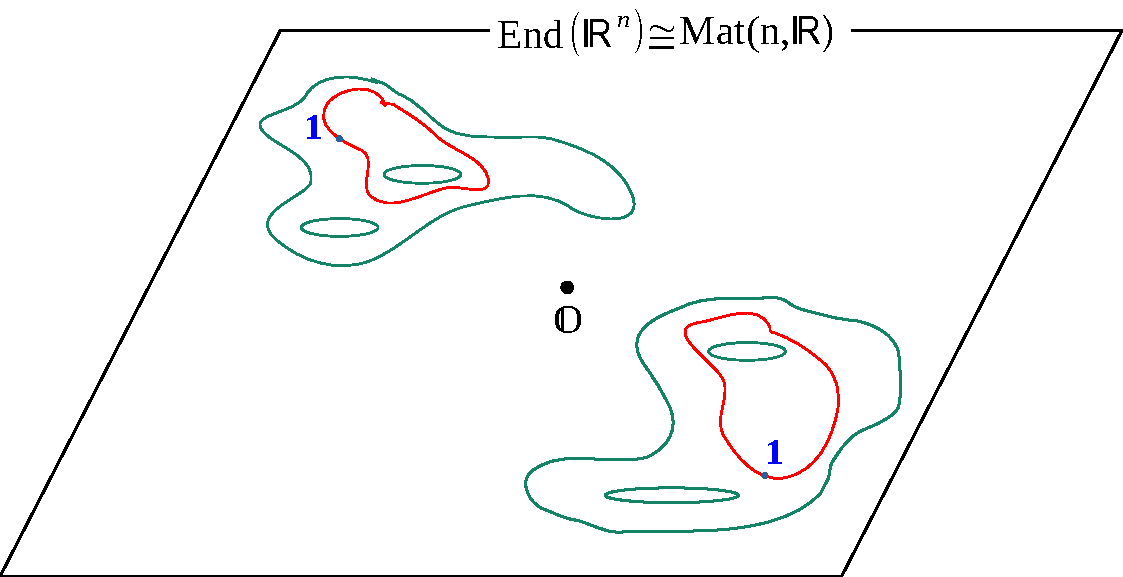
\includegraphics{images/buchi.pdf}
    \caption*{}
    \labfig{buchi}
\end{figure}
{\fontencoding{U}\fontfamily{futs}\selectfont\char 66\relax} The picture is not faithful! This is typically of \textbf{odd} dimensions. $\text{dim}\textrm{GL}(\mathbb{R}^n)=\text{dim End}(\mathbb{R}^n)=n^2$. Once we fix a condition, e.g. orthogonality, we reduce the dimension because the constraint that $A^TA-\mathbb{1}=0$ corresponds to many equations. Therefore, we have to imagine that $\textrm{O}(n)$ is something of lower dimension: $\text{dim}\textrm{O}(n)<n^2$, both $\mathbb{1}$ and $-\mathbb{1}$ are in $\textrm{O}(n)$. The component whose determinant is 1 corresponds to the connected component containing the identity.\begin{marginfigure}
	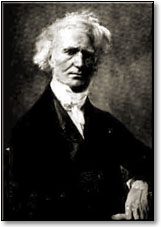
\includegraphics[width=1\linewidth]{images/Jacques_Binet.jpg}
	\caption[A portrait of Jacques Philippe Marie Binet]{From \href{https://commons.wikimedia.org/wiki/File:Jacques_Binet.jpg?uselang=it}{Wikimedia}: Jacques Philippe Marie Binet (February 2, 1786 – May 12, 1856) was a French mathematician, physicist and astronomer born in Rennes; he died in Paris, France, in 1856. He made significant contributions to number theory, and the mathematical foundations of matrix algebra which would later lead to important contributions by Cayley and others. In his memoir on the theory of the conjugate axes and of the moment of inertia of bodies he enumerated the principle now known as Binet's theorem. He is also recognized as the first to derive the rule for multiplying matrices in 1812, and Binet's formula expressing Fibonacci numbers in closed form is named in his honour, although the same result was known to Abraham de Moivre a century earlier.}
	\labfig{Binet}
\end{marginfigure}
\underline{\textbf{Terminology:}} \underline{n=3} is a special case, $\textrm{SO}(3)$ is the \textbf{group of rotations}. This will be our privileged example together with SU$(2).$

\underline{\textbf{Remark:}} definitions of $\textrm{O}(n)$ and $\textrm{SO}(n)$ depends on the \textbf{Euclidean structure} $E^n=(\mathbb{R}^n,(\dots|\dots))$:
\begin{align*}
(\dots,\dots):\mathbb{R}^n\times\mathbb{R}^n&\xrightarrow[]{}\mathbb{R}\\
              (v\underset{\mathclap{\tikz \node {$\uparrow$} node [below=1ex] {\footnotesize pair };}},w) &\mapsto (v\underset{\mathclap{\tikz \node {$\uparrow$} node [below=1ex] {\footnotesize inner product };}}|w)
\end{align*}
This is bilinear, symmetric and positive definite: $(v|v)\ge 0$, if $(v|v)=0\Rightarrow{}v=0$. For example, we could take the usual scalar product:
\[
(v|w)=\sum_{i,j=1}^n\delta_{ij}v^iw^j
\]
Once we fix the Euclidean structure we have the notion of \textbf{transpose} since it is the analogue of the adjoint but with respect to a bilinear, symmetric product (instead of a sesquilinear, hermitian product):
\[
(v|Aw)=({\color{red}A^T}v|w) \quad \forall\; v,w\in\mathbb{R}^n
\]
We want to emphasize that the definition of transpose depends on the scalar product in $\mathbb{R}^n$. The usual transpose is the one for the ordinary scalar product, but one might consider other cases, e.g by replacing $\delta_{ij}$ with a symmetric positive definite metric we have another scalar product and therefore we have to define the transpose with respect to that. We could make a step forward and consider generalized orthogonal groups with respect to metrics which are \textbf{not} positive defined. This is particularly relevant in the Physics Department since we know that the Lorentzian metric is not positive defined.
\end{document}